\documentclass[10pt]{report}
\usepackage[utf8]{inputenc}
\usepackage[italian]{babel}
\usepackage{multicol}
\usepackage[bookmarks]{hyperref}
\usepackage[a4paper, total={18cm, 25cm}]{geometry}
\usepackage{graphicx}
\usepackage{xcolor}
\usepackage{textcomp}
\graphicspath{ {./img/} }
\usepackage{listings}
\usepackage{makecell}
\usepackage{qtree}
\usepackage{pgfplots}
\usepackage{tikz}
\usepgflibrary{shapes}
\usepgfplotslibrary{fillbetween}
\definecolor{backcolour}{RGB}{255,255,255}
\definecolor{codegreen}{RGB}{27,168,11}
\definecolor{codeblue}{RGB}{35,35,205}
\definecolor{codegray}{RGB}{128,128,128}
\definecolor{codepurple}{RGB}{205,35,56}
\lstdefinestyle{myPython}{
	backgroundcolor=\color{backcolour},   
	commentstyle=\color{codegreen},
	keywordstyle=\color{codeblue},
	numberstyle=\tiny\color{codegray},
	stringstyle=\color{codepurple},
	basicstyle=\small\ttfamily,
	breakatwhitespace=false,         
	breaklines=true,                 
	captionpos=b,                    
	keepspaces=true,                 
	numbers=left,                    
	numbersep=2pt,                  
	showspaces=false,                
	showstringspaces=false,
	showtabs=false,                  
	tabsize=2,
	language=python
}
\newcommand*\triangled[1]{\tikz[baseline=(char.base)]{
            \node[regular polygon, regular polygon sides=3,draw,inner sep=1pt] (char) {#1};}}
            
\usepackage{fancyhdr}
\pagestyle{fancy}
\renewcommand{\headrulewidth}{0pt}
\fancyhead{}
\fancyfoot[L]{Telegram: \texttt{@fexed}}
\fancyfoot[R]{Github: \texttt{fexed}}
\begin{document}
\title{Intelligent Systems for Pattern Recognition}
\author{Federico Matteoni}
\date{A.A. 2021/22}
\renewcommand*\contentsname{Index}

\maketitle
\tableofcontents
\pagebreak
\section{Introduction}
Prof.s: Davide Bacciu and Antonio Carta
\paragraph{Objectives} Train ML specialists capable of: designing novel learning models, developing pattern recognition applications using ML, developing intelligent agents using \textbf{Reinforcement Learning}.\\
We're referring to images and signals, but not limited to that: practical applications.\\
Focusing on challenging and complex data: \textbf{machine vision} (noisy, hard to interpret, semantically rich\ldots) and \textbf{structured data} (relational information: sequences, trees, graphs\ldots)\\
Natural Language Processing will be used as an example, but will not be the focus of this course.
\paragraph{Methodology-Oriented Outcomes} Gain in-depth knowledge of advanced machine learning models, understanding the underlying theory. This gives the ability to read and understand and discuss research works in the field.
\paragraph{Application-Oriented Outcomes} Learn to address modern pattern recognition applications, gain knowledge of ML, PR and RL libraries and be able to develop an application using ML and RL models.
\paragraph{Prerequisites} Knowledge of ML fundamentals, mathematical tools for ML and Python.
\section{Pattern Recognition}
Automated recognition of meaningful patterns in noisy data.
\paragraph{Origins} 
\paragraph{Viola-Jones Algorithm} Framework for face recognition. Sum pixel in white area and subtract those in the black portion. The VJ algorithm positions the masks on the image and combines the responses (training set of $\simeq$5k images with hand-aligned filters)
\paragraph{An historical view} \begin{enumerate}
	\item Identification of distinguishing features of the object/entity (\textbf{feature detection})
	\item Extraction of features for the defining attributes (\textbf{feature extraction})
	\item Comparison with known patterns (\textbf{matching})
\end{enumerate}
Basically, lots of time spent hand-engineering the best data features.
\paragraph{A modern view}
Data is thrown into a neural network. A single stage process with a data crushing-and-munching neural network spitting out prediction, which encapsulates the three historical steps. But the time is now spent in fine-tuning the neural network.
\paragraph{The deep learning Lego} Creating applications by putting together various combinations of CNN and LSTM modules.
\subsection{Signals}
Signals are time series: a sequence of measurements in time. Examples of sources are: medicine, finance, geology, IoT, biometrics\ldots
\paragraph{Formalization} A time series x is a sequence of measurements in time $t$
$$\hbox{x} = x_0,\ldots,x_N$$
where $x_t$ or $x(t)$ is the measurement at time $t$.
\begin{list}{}{}
	\item Observation can be at \textbf{irregular} time intervals.
	\item We assume \textbf{weakly stationary} (or second-order stationary) data\begin{list}{}{}
		\item $\forall\:t\:\:E[x_t] = \mu$
		\item $\forall\:t$ Cov$(x_{t+\tau},x_t) = \gamma_\tau$ with $\gamma$ depending only on the lag $\tau$
	\end{list}
\end{list}
\paragraph{Goals}\begin{list}{}{}
	\item \textbf{Description}
	\item \textbf{Analysis}: identify and describe dependencies in data
	\item \textbf{Prediction}: forecast next values given information up to $t$
	\item \textbf{Control}: adjust parameters of the generative process to make the time series fit a target
\end{list}
\paragraph{Key Methods}\begin{list}{}{}
	\item \textbf{Time domain analysis}: assesses how a signal changes over time (correlation, convolution, auto-regressive models)
	\item \textbf{Spectral domain analysis}: assesses the distribution of the signal over a range of frequencies (Fourier analysis, wavelets)
\end{list}
\subsubsection{Time Domain Analysis}
\paragraph{Mean} $$\hat\mu=\frac{1}{N}\sum_{t=1}^N x_t$$
Can be used to subtract mean from values and "standardize" the two series.
\paragraph{Autocovariance} For lag $-N\leq \tau \leq N$
$$\hat\gamma_x(\tau) = \frac{1}{N}\sum_{t=1}^{N-|\tau|} (x_{t+|\tau|}-\hat\mu)(x_t - \hat\mu)$$
\paragraph{Autocorrelation} The correlation of a signal with itself. $$\hat\rho_x(\tau)=\frac{\hat\gamma_x(\tau)}{\hat\gamma_x(0)}$$
We can compute this with every possible $\tau$, finding the max/min which gives the $\tau$ where the autocorrelation is max/min, which means the lag where the signal starts repeating itself. The lags near zero typically dominates, so we want the maximum lag reasonably far from 0.
\subparagraph{Autocorrelation plot} It's a revealing view on time series statistics.
\paragraph{Cross-Correlation} A measure of similarity of x$_1$ and x$_2$ as a function of a time lag $\tau$ $$\phi_{\hbox{x}_1\:\hbox{x}_2}(\tau)=\sum_{t = \max\{0,\tau\}}^{\min\{(T_1 - 1 + \tau), (T_2 - 1)\}} \hbox{x}_1(t-\tau)\cdot \hbox{x}_2(t)$$
\subparagraph{Normalized cross-correlation} Returns an amplitude independent value
$$\overline{\phi}_{\hbox{x}_1\:\hbox{x}_2}(\tau) = \frac{\phi_{\hbox{x}_1\:\hbox{x}_2}}{\sqrt{\sum_{t=0}^{T_1-1}(x_1(t))^2\cdot\sum_{t=0}^{T_2-1}(x_2(t))^2}} \in [-1,+1]$$
With $\overline{\phi}_{\hbox{x}_1\:\hbox{x}_2}(\tau) = +1$ mean that the two time series have the exact same shape if aligned at time $\tau$. Nearing $-1$ we get the maximum anticorrelation, same shape but opposite sign. Near 0 we get that the two signals are completely \textbf{linearly} uncorrelated.\\
Note that we measure \textbf{linear correlation}.\\\\
Cross correlation looks like the convolution $$(f * g)[n]=\sum_{t=-M}^M f(n-t)g(t)$$ but we have a flipped sign ($n-t$ instead of $t-\tau$).\\
Cross-correlation is not symmetric, whereas convolution is ($f * g = g * f$).
\paragraph{Autoregressive Process} A timeseries autoregressive process (AR) of order $K$ is the linear system $$x_t = \sum_{k=1}^K \alpha_k x_{t-k} + \epsilon_t$$\begin{list}{}{}
	\item Autoregressive means $x_t$ regresses on itself
	\item $\alpha_k \Rightarrow$ linear coefficients$\:|\:|\alpha|<1$
	\item $\epsilon_t\Rightarrow$ sequence of independent and identically distributed values with mean 0 and fixed variance.
	\item We look backward $K$ steps, so limited memory.
\end{list}
\paragraph{ARMA} Autoregressive with Moving Average process $$x_t = \sum_{k=1}^K \alpha_k x_{t-k} + \sum_{q=1}^Q \beta_q\epsilon_{t-1}+\epsilon_t$$
\begin{list}{}{}
	\item With $\epsilon_t$ Random white noise (again)
	\item The current time series values is the result of a regression on its past values plus a term that depends on a combination of stochastically uncorrelated information
\end{list}
\paragraph{Estimating Autoregressive Models} Need to estimate: the values of the linear coefficients $\alpha_t$ and $\beta_t$ and the order of the autoregressor $K$ and $Q$\\
Estimation of the $\alpha$, $\beta$ is performed with the Levinson-Durbin Recursion (\texttt{levinson(x, K)} in matlab, and included in several Python modules).\\
The order is often estimated with a Bayesian model selection criterion, choosing the largest $K$ and $Q$ possible. E.g.: BIC, AIC\ldots\\
The set of autoregressive parameters $\alpha_{i,1},\ldots,\alpha_{i,K}$ fitted to a specific time series x$_i$ is used to confront it with other time series. Same thing for $\beta$ so we can use $\alpha$ for both sets.
\paragraph{Comparing time series by AR}\begin{list}{}{}
	\item timeseries clustering: $d(\hbox{x}_1,\hbox{x}_2)=\|\alpha_1-\alpha_2\|_M^2$
	\item novelty/anomaly detection: $\hbox{TestErr}(x_t,\hat{x}_t)<\xi$ with $\hat{x}_t$ being the AR predicted value.
\end{list}
\subsubsection{Spectral Domain Analysis}
Analyze the time series in the frequency domain. Key idea: decomposing the time series into a linear combination of sines and cosines with random and uncorrelated coefficients. So a \textbf{regression on sinusoids} with Fourier analysis.
\paragraph{Fourier Transform} Discrete Fourier Transform (DFT): transform a time series from the time domain to the frequency domain. Can be easily inverted back to the time domain.\\
Useful to handle periodicity in the time series: seasonal trends, cyclic processes\ldots
\paragraph{Representing functions} We know that, given an orthonormal system for $E$ we can use linear combinations of the basis $\{e_1,\ldots,e_k\}$ to represent any function $f\in E$ $$\sum_{k=1}^\infty \langle f,e_k\rangle e_k$$
Given the orthonormal system $$\{\frac{1}{\sqrt{2}}, \sin(x),\cos(x),\sin(2x),\cos(2x),\ldots\}$$
then the linear combination above becomes the Fourier series 
$$\frac{a_0}{2}+\sum_{k=1}^\infty\left(a_k\cos(kx)+b_k\sin(kx)\right)$$
\paragraph{Representing function in Complex space} Using $\cos(kx)-i\:\sin(kx) = e^{-ikx}$ with $i=\sqrt{-1}$ we can rewrite the Fourier series as $$\sum_{k=-\infty}^\infty c_k e^{ikx}$$
on the orthonormal system $$\{1,e^{ix},e^{-ix},e^{2ix},e^{-2ix},\ldots\}$$
\paragraph{Representing Discrete Time Series} Consider x of length $N$ and $x_n\in R$. Using the exponential formulation, the orthonormal system is finite, from $e_0$ to $e_{N-1}$ each $\in C^N$\\
The $n$-th component of the $k$-th vector is $$[e_k]n=e^{\frac{-2\pi ink}{2}}$$
\paragraph{Discrete Fourier Transform} Given a time series x = $x_0,\ldots,x_{N-1}$ its DFT is the sequence $$\hbox{Spectral domain}\:\:\:X_k = \sum_{n=1}^{N-1}x_ne^{\frac{-2\pi ink}{N}}\:\:\:\hbox{Time domain}$$
And can be inverted $$x_k = \frac{1}{N}\sum_{k=1}^{N-1}X_ke^{\frac{2\pi ink}{N}}$$
\paragraph{Basic Spectral Quantities in SFT}
\begin{list}{}{}
	\item Amplitude $A_k = |X_k| = \sqrt{Re^2(X_k)+Im^2(X_k)}$
	\item Power $P_k = \frac{|X_k|^2}{N}$, more used in reality and under some conditions this is a reasonable estimate of the power spectral density
\end{list}
\paragraph{DFT in Action} We use the DFT elements $X_1,\ldots,X_K$ as representation of the signal to train the predictor/classifier.\\
This representation can reveal patterns that are not clear in the time domain.
\subsection{Image Processing}
Bidimentional series. Basically same approach to signals.
\subsubsection{Descriptors}
An image is a matrix of pixel intensities or color values (RGB). There are other representations, not interesting for this course. CIE-LUV often used in image processing due to perceptual linearity (image difference is more coherent)
\paragraph{Machine Vision Applications} For example region of interest, or object classification.\\
Even pixel-level tasks, for example image segmentation (regions of the image) or semantic segmentation (classifying regions of the image).\\
Up one level of abstraction: automated image captioning, requiring identifying objects, generating sentences and ranking those sentences.
\paragraph{Key Questions}
\begin{list}{}{}
	\item How to represent visual information? It has to be:\begin{list}{}{}
		\item Informative, carrying all the information
		\item Invariant to photometric (different illuminations) and geometric transformation (position in the picture, rotation\ldots)
		\item Efficient for indexing and querying
	\end{list}
	\item How to identify informative parts?\begin{list}{}{}
		\item Whole image is generally not a good idea
		\item Must lead to good representations
	\end{list}
\end{list}
\paragraph{Image Histograms} One of the first answer. Describes the distribution of some visual information on the whole image: colors, edges, corners\ldots depending on the goals.\begin{list}{}{}
	\item \textbf{Color Histograms}, one of the earliest image descriptors.\\
	Count the number of pixels of a given color (normalize!). We need to discretize and group the RGB colors.\\
	Any information concerning shapes and position is lost. Two image with a random permutation of the same pixels produce the same color histograms.\\
	Images can be compared, indexed and classified based on their color histogram representation.\\
	Can be computed with OpenCV in Python.
\end{list}
\paragraph{Describing Local Image Properties} We need something less global, on a local level. Capturing information on image regions, extract \textbf{multiple local descriptors}: different location, different scale\ldots\\
Several approaches, typically performing convolution between a filter and the image region. Using filters sensitive to specific features we can extract many kind of information.
\paragraph{Localized Descriptors}
\begin{list}{}{}
	\item \textbf{Intensity Vector} The simplest form of localized descriptor: a vector $n\cdot m$ of the pixels of a single patch of the image with dimensions $n,m$. The vector can be normalized to make it invariant to intensity variations.\\
	But rotating gives a different vector. A more robust representation is an histogram of this vector.
	\item \textbf{Distribution-Based Descriptors} Represent local patches by histograms describing properties of the pixels in the patch. The simplest is an histogram of intensity values, but it's not invariant enough even if normalized.\\
	We want a descriptor invariant to illumination (normalization), scale (captured at multiple scale) and geometric transformations (rotation invariant). We want locality, histogram based and invariant to geometric transformation.
\end{list}
\paragraph{SIFT} \textbf{Scale Invariant Feature Transform}\begin{enumerate}
	\item Center the image patch on a pixel $x,y$ of the image $I$
	\item Represent image at scale $\sigma$ (controls how close to look at the image)
	\item[] Convolve the image with a Gaussian filter with standard variation $\sigma$, basically computing average of pixels with the coefficient taken from a Gaussian distribution. With a smooth Gaussian, we artificially smooth the object, and vice versa. We can compute different versions of the image.
$$L_\sigma(x,y) = G(x,y,\sigma) * I(x,y)$$
$$G(x,y,\sigma) = \exp\left(-\frac{x^2+y^2}{2\sigma^2}\right)$$
	\item Compute the \textbf{gradient of intensity} in the patch, extracting magnitude $m$ and orientation $\Theta$ using finite differences.
\end{enumerate}
\subparagraph{Gaussian Filter of an Image}
\begin{center}
	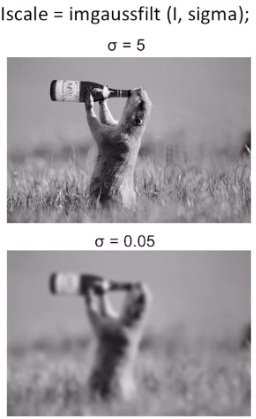
\includegraphics[scale=0.5]{1.png} 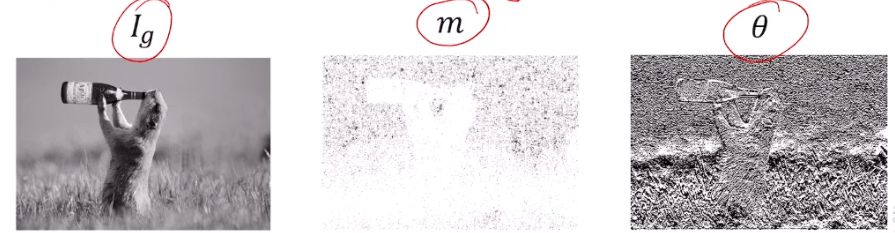
\includegraphics[scale=0.6]{2.png}
\end{center}
\pagebreak
\begin{list}{}{}
	\item[4.] Create \textbf{gradient histogram}\begin{list}{}{}
		\item 4$\times$4 gradient window
		\item Histogram of 4$\times$4 per window on 8 orientation bins
		\item Gaussian weighting on center keypoint (width = $1.5\sigma$)
		\item 4$\times$4$\times$8 = 128 descriptor size
	\end{list}
\end{list}
\begin{center}
	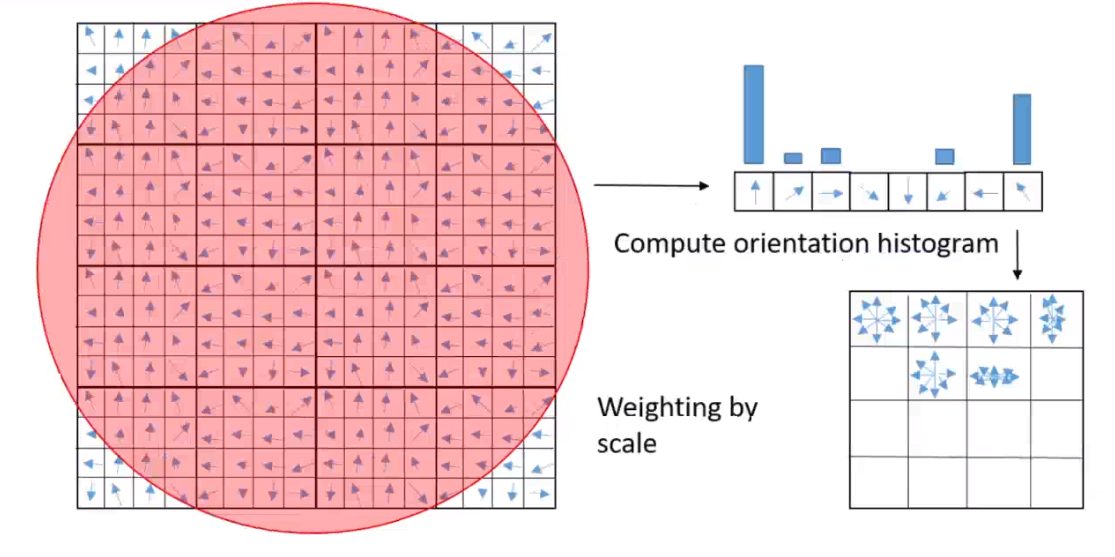
\includegraphics[scale=0.5]{3.png}
\end{center}
\subsubsection{Detectors}
\paragraph{Visual Feature Detector} Properties
\begin{list}{}{}
	\item \textbf{Repeatability} Detect the same feature in different image portions and different images, under different conditions (color, luminance\ldots). So with respect to translation, photometric changes, rotation, scaling and affine transformations (non-isotropic changes, for example the relative position of the camera)\ldots
\end{list}
\paragraph{Edge Detection} We need to find interesting points, talking about fundamental elements, basic components. One possible example are the edges of the image.\\
Reasoning in changes of intensity: edges are those points where the intensity changes.\begin{center}
	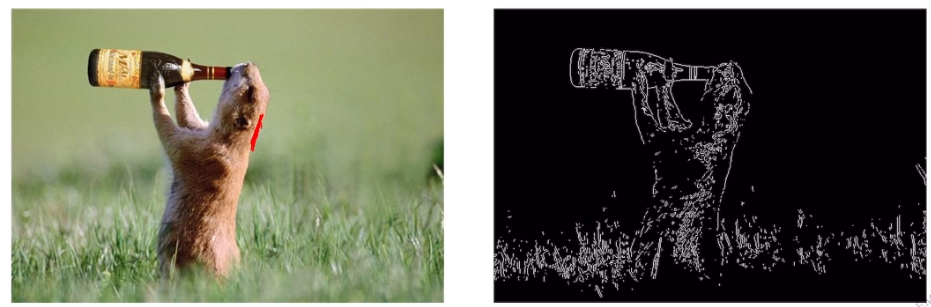
\includegraphics[scale=0.5]{4.png}
\end{center}
Typically using an edge detector filter on each pixel and turning pixels white or black by thresholding
\subparagraph{Edges and Gradients} The image gradient (graylevel) is $$\nabla I = \left[\frac{\partial I}{\partial x},\frac{\partial I}{\partial y}\right]$$ which is basically two images, gradient in both $x$ and $y$ directions. Edge are pixel regions where intensity gradient changes abruptly. The return of finite difference methods:
\begin{list}{}{}
	\item $G_x = \frac{\partial I}{\partial x} \simeq I(x+1,y)-I(x-1,y)$
	\item $G_y = \frac{\partial I}{\partial y} \simeq I(x,y+1)-I(x,y-1)$
\end{list}
\pagebreak
Edge detectors build on this idea combining with some smoothing: average on multiple pixels.
\subparagraph{Prewitt operators}
$$G_x = \left[\begin{array}{c c c }
+1&0&-1\\
+1&0&-1\\
+1&0&-1
\end{array}\right]\:\:\:\:\:G_y = \left[\begin{array}{c c c }
+1&+1&+1\\
0&0&0\\
-1&-1&-1
\end{array}\right]$$
\begin{center}
	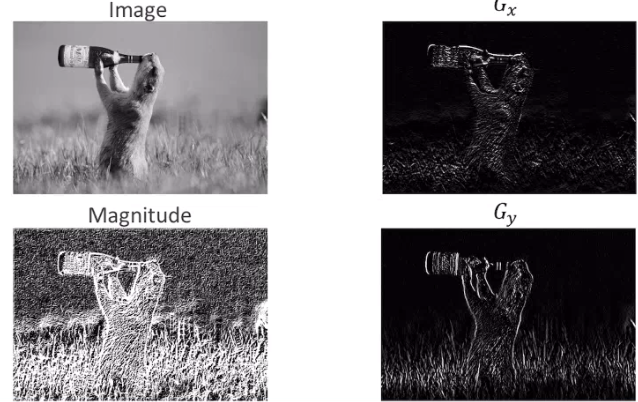
\includegraphics[scale=0.5]{5.png}
\end{center}
\subparagraph{Sobel Operator}
$$G_x = \left[\begin{array}{c c c }
+1&0&-1\\
+2&0&-2\\
+1&0&-1
\end{array}\right]\:\:\:\:\:G_y = \left[\begin{array}{c c c }
+1&+2&+1\\
0&0&0\\
-1&-2&-1
\end{array}\right]$$
Often with a constant $c\simeq \frac{1}{8}$ for scaling.
\begin{center}
	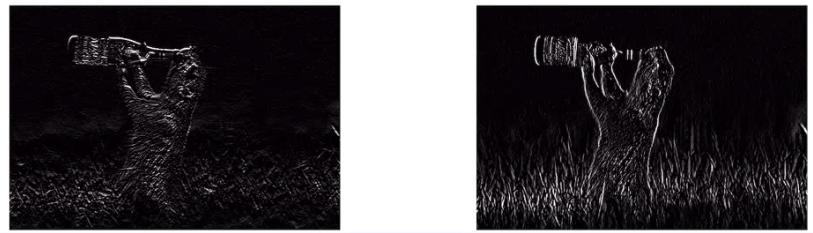
\includegraphics[scale=0.4]{6.png}
\end{center}
\paragraph{Blob Detection} Pixel regions with little gradient variability.\\
$g_\sigma(x,y)$ has maximum response when centered on a circle of radius $\sqrt{2}\sigma$, with $\sigma$ being the scale of the gaussian.\\
Laplace of Gaussian (LoG):
$$\nabla^2g_\sigma(x,y)=\frac{\partial^2g_\sigma}{\partial x^2} + \frac{\partial^2g_\sigma}{\partial y^2}$$
Typically using a scale normalized response
$$\nabla^2_{norm}g_\sigma(x,y)=\sigma^2\left(\frac{\partial^2g_\sigma}{\partial x^2} + \frac{\partial^2g_\sigma}{\partial y^2}\right)$$
\begin{enumerate}
	\item Convolve image with a LoG filter at different scales $\sigma = k\sigma_0$ by varying $k$ with a starting $\sigma_0$
	\item Find maxima of squared LoG responses:
	\begin{list}{}{}
		\item Find maxima on space-scale: focus on a scale and find maxima
		\item Find maxima between scales: do the same for all the scales and pick the maxima
		\item Threshold
	\end{list}
\end{enumerate}
The LoG can be approximated by the Difference of Gaussians (DoG) for efficiency, so to reuse part of the computations.
$$g_{k\sigma_0}(x,y) - g_{\sigma_0}(x,y) \simeq (k-1)\sigma_0^2\nabla^2g_{(k-1)\sigma_0}$$
SIFT uses LoG.
\paragraph{Affine Detectors} Laplacia-based detectors are invariant to scale thanks to the maximization in scale-space. Still not invariant to affine-transformation.
\begin{center}
	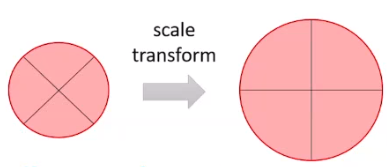
\includegraphics[scale=0.5]{7.png}\\
	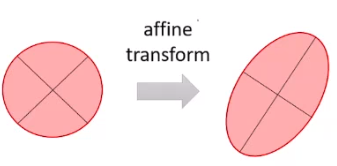
\includegraphics[scale=0.5]{8.png}
\end{center}
\paragraph{MSER} Maximally Stable Extremal Regions\\
Extract covariant regions (blobs) that are stable connected components of intensity sets of the image. Interesting areas stay the same at different thresholds: stable with respect to variations in luminance, not scale dependent and doesn't assume circular regions. The key idea is to \textbf{take the blobs} (\textbf{extremal regions}) \textbf{which are nearly the same through a wide range of intensity thresholds}.\\
Blobs are generated (locally) by binarizing the image over a large number of thresholds:\begin{list}{}{}
	\item Invariance to affine transformation of image intensities
	\item Stability (they are stable on multiple thresholds)
	\item Multi-scale (connected components are identified by intensity stability not by scale)
	\item Sensitive to local lightning effects, shadows\ldots
\end{list}
\subparagraph{Intuitions on MSER} Generate frames from the image by thresholding it on all graylevels.\\
Capture those regions that from a small seed of pixel grow to a stably connected region. Stability is assessed by looking at derivatives of region masks in time (most stable $\Rightarrow$ minima of connected region variation).
\paragraph{Image Segmentation} The process of partitioning an image into a set of homogeneous pixels, hoping to match objects or their subparts.\\
A naive approach: straighten the image in a $N\cdot M$ vector and use it as a dataset for K-means.\\
\subparagraph{Ncut} Normalized cuts
\begin{center}
	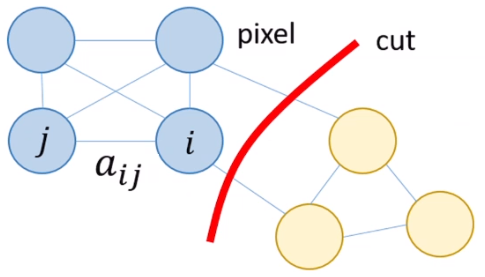
\includegraphics[scale=0.5]{9.png}
\end{center}
With each node being a pixel: an image is a graph. $a_{ij}$ is the affinity between pixels at a certain scale $\sigma$. A cut of $G$ is the set of edges such whose removal makes $G$ a disconnected graph. Breaking the graph into pieces by cutting edges of low affinity.\\
The normalized cut problem is NP-hard, approximate solution as an eigenvalue problem. But the eigenvalue decomposition it's really intractable with big images. We need to reduce the number of pixels. We can use \textbf{superpixels}: clustering the pixels with K-means (perhaps with different $K$) and using the clusters as nodes for segmentation algorithms (Ncut, Markov Random Fields\ldots). We can do multiscale superpixeling and segmenting at different scales, different policies\ldots\\
\subsubsection{Conclusion}
Image processing is a lot about convolutions: linear masks to perform gradient operations, gaussian functions to apply scale changes (zooming in and out). Computational efficiency is a driving factor: convolution in Fourier domain, superpixel, lightweight feature detectors\ldots
\subsection{Wavelets}
\paragraph{Limitations of DFT} Sometimes we might need localized frequencies rather than global frequency analysis.
\begin{center}
	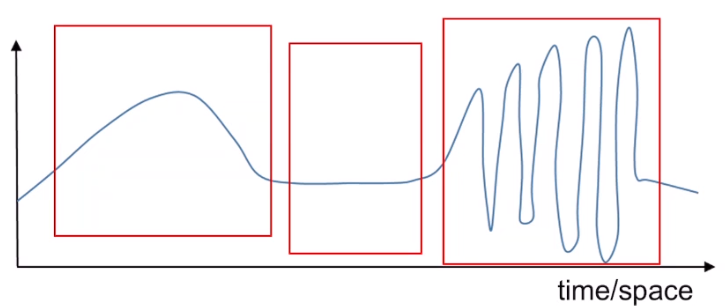
\includegraphics[scale=0.5]{10.png}
\end{center}
We slice the signal in "time slots" in time analysis and "frequency slots" in frequency analysis. In wavelet analysis you do both.\begin{center}
	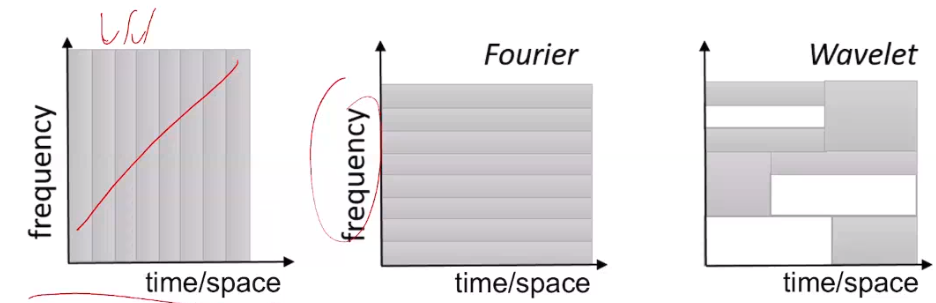
\includegraphics[scale=0.33]{11.png}\\
	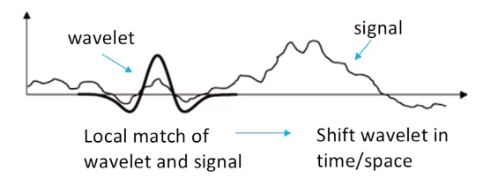
\includegraphics[scale=0.5]{12.png}
\end{center}
\begin{enumerate}
	\item Scale and shift original signal
	\item Compare signal to a wavelet
	\item Compute coefficient of similarity
\end{enumerate}
Split the signal with an orthonormal basis generate by translation and dilation of a mother wavelet $$\sum_t \hbox{x}(t)\phi_{j,k}(t)$$
Terms $k,j$ regulate scaling and shifting of the wavelet
$$\phi_{t,k}(\hbox{x}) = 2^{\frac{k}{2}}\phi\left(\frac{t-j2^k}{2^k}\right)$$
With many different options for the mother wavelet $\phi$
\begin{center}
	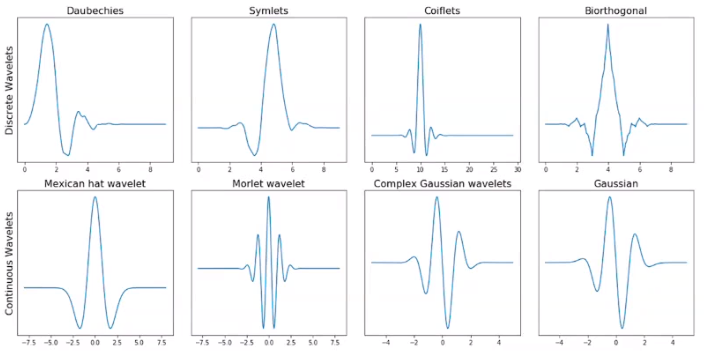
\includegraphics[scale=0.5]{13.png}
\end{center}
Scaling and dilation is akin to a sort of frequency: high scale mean stretched wavelet with slowly changing coarse feature and low frequency, while low scale compressed wavelet with rapidly changing details and high frequency.
\paragraph{DWT} Discrete Wavelet Transform: uses a finite set of scales and shifts rather than "any possible value" as in the continuous wavelet transform.
\section{Generative and Graphical Models}
Generative referring to the probability we learn: if we know the distribution probability of data we can generate new data.\\
Graphical referring to graphical formalisms that describe in a syntetic way the structures we'll see.
\paragraph{Generative Learning} ML models that represent knowledge inferred from data under the form of probabilities:
\begin{list}{}{}
	\item Probabilities can be sample: new data can be generated
	\item Supervised, unsupervised, weakly supervised tasks
	\item More easily incorporate prior knowledge on data and tasks
	\item Interpretable knowledge (how data is generated)
\end{list}
The majority of modern tasks comprises large number of variables\begin{list}{}{}
	\item Modeling the joint distribution of all variables can become impractical
	\item Exponential size of the parameter space
	\item Computationally impractical to train and predict
\end{list}
\paragraph{Representation} Graphical models are a compact way to represent exponentially large probability distributions. Encode conditional independence assumptions, and different classes of graph structures imply different assumptions/capabilities.
\paragraph{Inference} How to query (predict with) a graphical model? Probability of unknown $X$ given observations $d$, $P(X\:|\:d)$, the \textbf{most likely hypothesis} (parameters) $X$.
\paragraph{Learning} Find the right model parameters.
\paragraph{Representation} A graph whose nodes are random variables and edges represent probabilistic relationships between the variables.\\
Different classes of graphs:
\begin{list}{}{}
	\item Directed edges express \textbf{causal relationships}
	\item Undirected edges express \textbf{soft constraints}, values cannot change independently
	\item \textbf{Dynamic models}, graphs subject to structure changes to reflect dynamic processes. For example RNNs: recurrent neural networks are unfolded using weight sharing, producing a dynamic model.
\end{list}
\paragraph{In Deep Learning} Bayesian learning necessary to understand Variational Deep Learning.
\begin{center}
	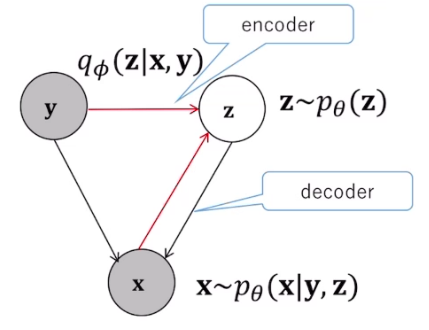
\includegraphics[scale=0.5]{14.png}
\end{center}
\paragraph{Generate new knowledge} Complex data can be generated if the model is powerful enough to capture its distribution.
\subsection{Probability Refresher}
\texttt{todo}
\subsubsection{Inference} Bayesian: consider all hypothesis weighted by their probabilities
$$P(X\:|\:d)=\sum_i P(X\:|\:h_i)P(h_i\:|\:d)$$
MAP (Maximum a-Posteriori): infer $X$ from $P(X\:|\:h_{MAP})$ where $h_{MAP}$ is the maximum a-posteriori hypothesys given $d$
$$h_{MAP} = \arg\max_{h\in H} P(h\:|\:d) = \arg\max_{h\in H} P(d\:|\:h)P(h)$$
ML assuming uniform prioris $P(h_i)=P(h_j)$ yields the maximum likelihood (ML) estimate $P(X\:|\:h_{ML})$ $$h_{ML} = \arg\max_{h\in H} P(d\:|\:h)$$
Any probability can be obtained from the Joint Probability Distribution $P(X_1,\ldots,X_n)$ by marginalization but at an exponential cost (e.g. $2^{n-1}$ for a marginal distribution from binary RV)
\subsection{Graphical Models}
Compact graphical representation for exponentially large joint distributions: simplifies marginalization and inference algorithms, allowing to \textbf{incorporate prior knowledge} concerning causal relationships and associations between random variables.\begin{list}{}{}
	\item Directed graphical models (Bayesian Networks)
	\item Undirected graphical models (Markov Random Fields)
\end{list}
\subsubsection{Bayesian Networks} 
\begin{multicols}{2}
Directed Acyclic Graphs (DAG) $G = (V,E)$\begin{list}{}{}
	\item Nodes $v\in V$ represent random variables\\
	Shaded $\Rightarrow$ observed, empty (like $Y_3$) $\Rightarrow$ unobserved
	\item Edges $e\in E$ describe the conditional independence relationships
\end{list}
\columnbreak
\begin{center}
	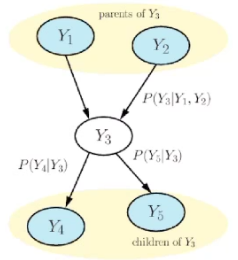
\includegraphics[scale=0.5]{15.png}
\end{center}
\end{multicols}
\paragraph{Conditional Probability Tables} CPTs are local to each node and describe the probability distribution \textbf{given its parents}.
$$P(Y_1,\ldots,Y_n) = \prod_{i=1}^N P(Y_i\:|\:\hbox{Parents}(Y_i))$$
\paragraph{Plate notation} If the same causal relationship is replicated for a number of variables, we can compactly represent it with plate notation.
$$P(Y_1,\ldots,Y_N,C) = P(C)\prod_{i=1}^N P(Y_i\:|\:C)$$
\begin{center}
	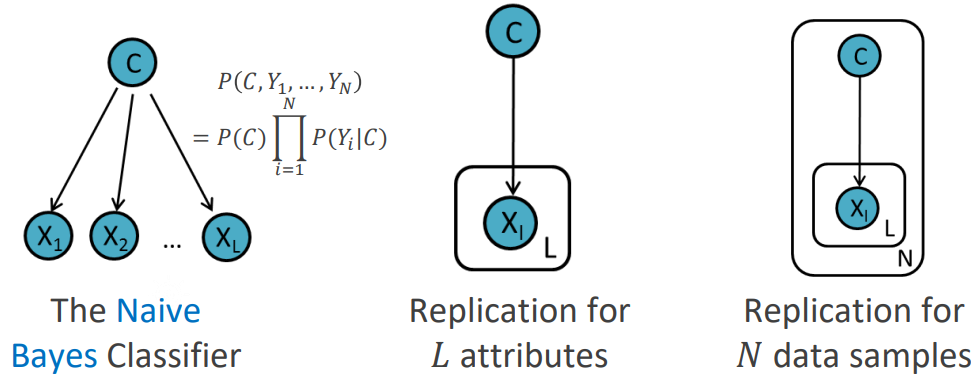
\includegraphics[scale=0.5]{16.png}
\end{center}
\paragraph{Full-Plate Notation}
Boxes denote replication for a number of times (denoted by the letter in the corner). Shaded nodes are observed variables, empty nodes are unobserved latent variables.\\
Black dots (optional) identify model parameters.
\begin{center}
	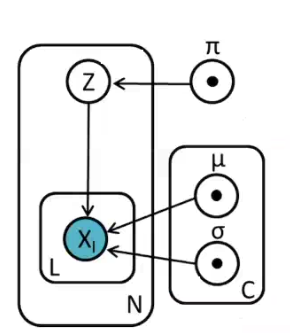
\includegraphics[scale=0.5]{17.png}
\end{center}
\subsubsection{Markov Random Fields}
\begin{center}
	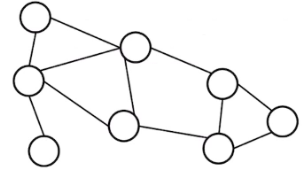
\includegraphics[scale=0.5]{18.png}
\end{center}
Undirected graph $G = (V,E)$ (a.k.a. Markov Networks). Also with shaded/empty nodes to denote observed/unobserved variables.\\
Edges $e\in E$ represent bidirectional dependencies between variables (constraints).\\
Often arranged in a structure that is coherent with the data/constraint we want to model.\\
Often used in image processing to impose spatial constraints (e.g. smoothness)
\subsection{Conditional Independence and Causality}
Can we reason on the structure of the graph to infer direct/indirect relationships between random variables?
\paragraph{Local Markov Property} Each node (random variable) is conditionally independent of all its non-descendants given a joint state of its parents. $$Y_v\perp Y_{V\setminus \hbox{Children(v)}}\hbox{ given }Y_{\hbox{Parent}(v)}\:\:\forall\:v\in V$$
There are substructures in the Bayesian networks with which we can build everything.
\paragraph{Markov Blanket} A Markov blanket $Mb(A)$ of a node $A$ is the minimal set of vertices that isolates/shields the node from the rest of the Bayesian network. If I know the variables in $Mb(A)$ then I know everything I need to know about $A$\begin{center}
	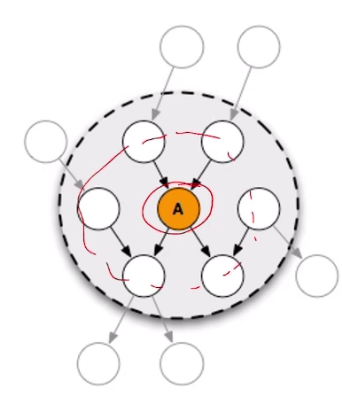
\includegraphics[scale=0.5]{19.png}
\end{center}
Taking only the parents it's not sufficient, we need also the children and the co-parents (nodes that are parents of one of my children). So it contains parents, children and children's parents.
$$P(A\:|\:Mb(A), Z) = P(A\:|\:Mb(A))\:\:\forall\:Z\not\in Mb(A)$$
\paragraph{Joint Probability Factorization} An application of the chain rule and local Markov property.\begin{enumerate}
	\item Pick a topological ordering of the nodes
	\item Apply chain rule following the order
\end{enumerate}
\paragraph{Sampling of a Bayesian Network} A BN describes a generative process for observations.
\begin{enumerate}
	\item Pick a topological ordering of the nodes
	\item Generate data by sampling from the local condition probabilities following this order
\end{enumerate}
Generate $i$th sample for each variable, example $s_i\simeq P(S)$, $h_i\simeq P(H\:|\:S=s_i)$
\subsection{Fundamental Bayesian Network Structures}
Three fundamental substructures that determine the conditional independence relationships in a Bayesian network.
\paragraph{Tail to Tail} Common cause \begin{center}
	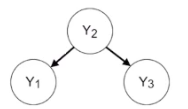
\includegraphics[scale=0.75]{20.png}
\end{center}
$$P(Y_1,Y_3\:|\:Y_2)=P(Y_1\:|\:Y_2)P(Y_3\:|\:Y_2)$$
If $Y_2$ is unobserved, then $Y_1,Y_3$ are marginally dependent $Y_1\not\perp Y_3$\\
If $Y_2$ is observed, $Y_1,Y_3$ become conditionally independent $Y_1\perp Y_3\:|\:Y_2$ (the path between $Y_1,Y_3$ is blocked by the observed (shaded) $Y_2$)
\paragraph{Head to Tail} Causal Effect \begin{center}
	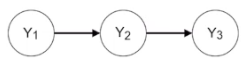
\includegraphics[scale=0.75]{21.png}
\end{center}
$$P(Y_1,Y_3\:|\:Y_2)=P(Y_1)P(Y_2\:|\:Y_1)P(Y_3\:|\:Y_2)=P(Y_1\:|\:Y_2)P(Y_3\:|\:Y_2)$$
Same behavior as before!\\
If $Y_2$ is unobserved, then $Y_1,Y_3$ are marginally dependent $Y_1\not\perp Y_3$\\
If $Y_2$ is observed, $Y_1,Y_3$ become conditionally independent $Y_1\perp Y_3\:|\:Y_2$ ($Y_2$ again blocks the path)
\paragraph{Heat to Head} Common effect\begin{center}
	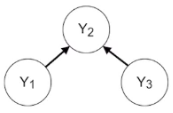
\includegraphics[scale=0.75]{22.png}
\end{center}
$$P(Y_1,Y_2,Y_3) = P(Y_1)P(Y_3)P(Y_2\:|\:Y_1,Y_3)$$
If $Y_2$ is unobserved, then $Y_1,Y_3$ are marginally independent $Y_1\perp Y_3$\\
If $Y_2$ is observed, then $Y_1,Y_3$ are conditionally dependent $Y_1\not\perp Y_3\:|\:Y_2$\\
If any $Y_2$ descendants is observed it unlocks the path.
\paragraph{Derived Conditional Independence Relationships} A Bayesian network represent the local relationship encoded by the 3 basic structures plus the derived relationships.\\\\
Given the same distribution I can have two different Bayesian Networks, which implies the same factorization.
\begin{center}
	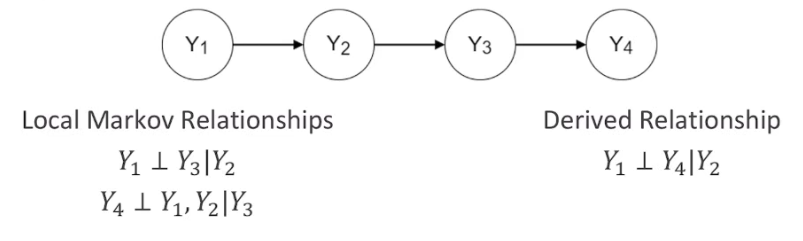
\includegraphics[scale=0.5]{23.png}
\end{center}
\paragraph{$d$-separation} Let $r = Y_1\leftrightarrow\ldots\leftrightarrow Y_2$ be an undirected path between $Y_1,Y_2$, $r$ is $d$-separated by $Z$ if there exist at least one node $Y_c\in Z$ for which path $r$ is blocked. With $Z$ being the set of variable for which we're assessing this separation.\\
In other words, this holds if at least one of the following holds:\begin{list}{}{}
	\item $r$ contains an head-to-tail structure $Y_i\rightarrow Y_c\rightarrow Y_j$ (or $Y_i\leftarrow Y_c\leftarrow Y_j$) and $Y_c \in Z$
	\item $r$ contains a tail-to-tail $Y_i\leftarrow Y_c\rightarrow Y_j$ and $Y_c \in Z$
	\item $r$ contains head-to-head $Y_i\rightarrow Y_c\leftarrow Y_j$ and neither $Y_c$ nor its descendants are in $Z$
\end{list}
Two nodes $Y_i,Y_j$ in a Bayesian Network $G$ are $d$-separated by $Z\subset V$ $\Leftrightarrow$ all undirected paths between $Y_i,Y_j$ are $d$-separated by $Z$ (denoted by $\hbox{Dsep}_G(Y_i,Y_j\:|\:Z)$)
\paragraph{Markov Blanket} The Markov Blanket $Mb(Y)$ is the minimal set of nodes which $d$-separates a node $Y$ from all other nodes (i.e. makes $Y$ conditionally independent of all other nodes in the Bayesian Network)
$$Mb(Y) = \{\hbox{Parents}(Y), \hbox{Children}(Y), \hbox{Parents}(\hbox{Children}(Y))\}$$
\paragraph{Are Directed Models Enough?} Bayesian Networks are used to model asymmetric dependencies. But Directed Models cannot express all conditional dependence relationships: expressing some precludes the expressions of others.\\
What if we want to model symmetric dependencies: bidirectional effects, spatial dependencies... we need \textbf{undirected approaches}. Directed models cannot represent some bidirectional dependencies in the distributions.
\subsection{Markov Random Fields}\begin{center}
	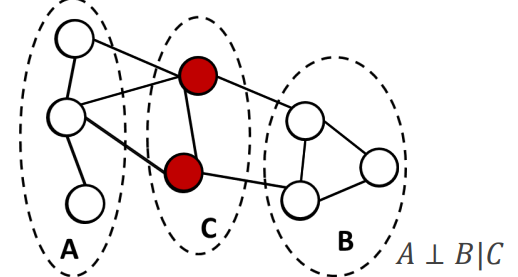
\includegraphics[scale=0.5]{24.png}
\end{center}
What is the undirected equivalent of $d$-separation in directed models? It's based on node separation: the two nodes in the middle separate the two lateral parts.\\
Node subsets $A,B\subset V$ are conditionally independent given $C\subset V\setminus \{A,B\}$ if all paths between nodes in $A$ and $B$ pass through at least one of the nodes in $C$.\\
The Markov Blanket of a node includes all and only its neighbors.
\paragraph{Joint Probability Factorization} What is the undirected equivalent? We seek a product of functions defined over a set of nodes associated with some local properties of the graph. Markov blanket tells that nodes that are not neighbors are conditionally independent given the remainder of the nodes.$$P(X_v,X_i\:|\:X_{V\setminus\{v,i\}}) = P(X_v\:|\:X_{V\setminus\{v,i\}})P(X_i\:|\:X_{V\setminus\{v,i\}})$$
Factorization should be chosen in a way that nodes $X_v$ and $X_i$ are not in the same factor: we use a well-known graph structure that includes only nodes that are pairwise connected.
\subparagraph{Clique} Subset of nodes $C$ in graph $G$ such that $G$ contains an edge between all pair of nodes in $C$. It's maximal if you cannot add more nodes.
\subparagraph{Maximal Clique Factorization} Define $X = X_1,\ldots,X_n$ as the random variables associated to the $N$ nodes of the undirected graph $G$ $$P(X)=\frac{1}{Z}\prod_C \psi(X_C)$$
$X_C$ are the random variables in the maximal clique $C$, $\psi(X_C)$ is the \textbf{potential function} over the maximal clique $C$ and $Z$ is the partition function ensuring normalization.
$$Z = \sum_X\prod_C\psi(X_C)$$
The partition function $Z$ is the computational bottleneck of undirected modes: $O(K^N)$ for $N$ discrete random variables with $K$ distinct values.
\paragraph{Potential Functions} Potential functions $\psi(X_C)$ are not probabilities, they express which configuration of the local variables are preferred. For example $\psi(X_1,X_2)=\left\{ \begin{array}{l l}
1&\hbox{if }X_1 = X_2\\
4&\hbox{if }X_2 = 2X_1\\
0&\hbox{otherwise}
\end{array}\right.$: you can hand-engineer feature functions.\\
If we restrict to strictly positive potential functions, the Hammersley-Clifford theorem provides guarantees on the distribution that can be repreesented by the clique factorization.
\paragraph{Boltzmann Distribution} A convenient and widely used strictly positive representation of the potential function is $$\psi(X_C)=e^{-E(X_C)}$$
where $E(X_C)$ is called \textbf{energy function}.
\subsubsection{From Directed to Undirected}
Straightforward when is linear.\\Requires some work with v-structures, e.g. \textbf{moralization} (a.k.a. marrying of the parents).\begin{center}
	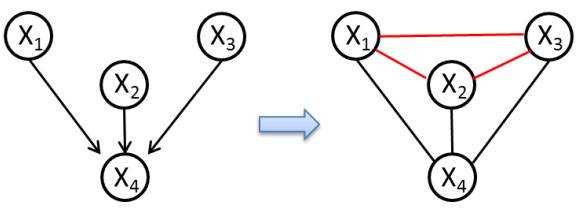
\includegraphics[scale=0.5]{25.png}
\end{center}
\subsection{Learning Causation from Data}
\paragraph{Learning with Bayesian Network}
\begin{center}
	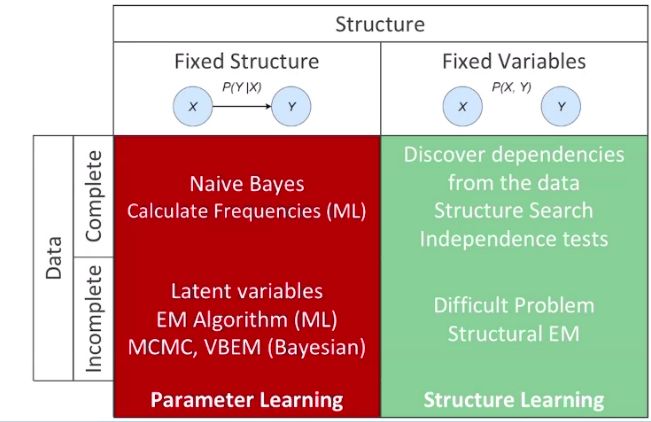
\includegraphics[scale=0.5]{26.png}
\end{center}
\paragraph{Structure Learning Problem} Observations are given for a set of fixed random variables, and network structure is not specified:\begin{list}{}{}
	\item Determine which arcs exist in the network (causal relationships)
	\item Compute Bayesian network parameters (conditional probability tables)
\end{list}
Determining causal relationships between variables entails deciding on arc presence and directing edges.
\subparagraph{Structure Finding Approaches}\begin{list}{}{}
	\item \textbf{Search and Score}\\A model selection approach, a search in the space of the graphs.\\
	Search the space Graph$(Y)$ of graphs $G_k$ that can be built on the random variables $Y = Y_1,\ldots,Y_N$, scoring each structure by $S(G_k)$ and returning the highest scoring graph $G^*$. So two fundamental aspects: the scoring function and the search strategy.\\
	\textbf{Scoring function}: two fundamental properties:\begin{list}{}{}
		\item Consistency: same score for graphs in the same equivalence class
		\item Decomposability: can be locally computed
	\end{list}
	Two approaches:\begin{list}{}{}
		\item Information theoretic: based on data likelihood plus some model-complexity penalization terms
		\item Bayesian: score the structures using a graph posterior (likelihood plus proper prior choice
	\end{list}
	\textbf{Search strategy}:\begin{list}{}{}
		\item Finding maximal scoring structures is NP complete
		\item Constrain search strategy: starting from a candidate structure we modify iteratively by local operations (edge/node addition/deletion). Each operation has a cost, so a cost optimization problem.
	\end{list}
	Constrain search space can be\begin{list}{}{}
		\item Known node order: can reduce the search space to the parents of each node (Markov Blankets)
		\item Search in the space of structure equivalence classes
		\item Search in the space of node ordering
	\end{list}
	\item \textbf{Constraint Based}\\
	Tests of conditional independence $I(X_i,X_j\:|\:Z)$, constraining the network. Based on measures of association between two variables $X_i$ and $X_j$ given their neighbor nodes $Z$.\\
	\textbf{Testing strategy}:\begin{list}{}{}
		\item Choice of the testing order is fundamental in avoiding a super-exponential complexity.
		\item Level-wise testing: tests $I(X_i,X_j\:|\:Z)$ are performed in order of increasing size of the conditioning set $Z$ starting from $Z = \emptyset$ (PC algorithm)
		\item Node-wise testing: tests are performed on a single edge at the time, exhausting independence checks on all conditioning variables (TPDA algorithm)
		\item The nodes entering $Z$ are chosen in the neighborhood of $X_i,X_j$
	\end{list}
	\item \textbf{Hybrid}\\
	Model selection of constrained structures. Multi-stage algorithm combining previous approaches: independence tests to find a good sub-optimal skeleton as starting point, then search and score refining the skeleton.\\
	Max-Min Hill Climbing (MMHC) model: optimized constraint-based approach to reconstruct the skeleton, using the candidate parents in the skeleton to run a search and score approach.
\end{list}
\subsection{Hidden Markov Models}
\paragraph{Sequence}A sequence $y$ is a collection of observations $y_t$ where $t$ represent the position of the element according to a complete order (e.g. time)
$$y_1\rightarrow \ldots\rightarrow y_{t-1}\rightarrow y_t\rightarrow\ldots\rightarrow y_T$$
$$P(y_t\:|\:y_{t-1})$$
Also head-to-tail: observation at time $t$ is independent from $t=1,\ldots,t-1$: \textbf{first-order Markov assumption}.\\
Reference population is a set of independent and identically distributed sequences $y^1, \ldots, y^N$\\
Difference sequences generally have different lengths $T^1,\ldots,T^N$
\paragraph{Markov Chain} First-Order Markov Chain is a directed graphical model for sequences such that element $x_t$ only depends on %TODO
We have X = $x-1,\ldots,x_T$ that can be represented as 
$$x_1\rightarrow \ldots\rightarrow x_{t-1}\rightarrow x_t\rightarrow\ldots\rightarrow x_T$$
So we can write $$P(\hbox{X}) = P(x_1,\ldots,x_T) = P(x_1)\cdot\prod_{i=2}^T P(x_i\:|\:x_{i-1})$$
because $P(x_i\:|\:x_{i-1})$ is the same whenever the $t$.\\
$P(x_1)$ is the \textbf{prior distribution} ($x_1$ has nothing "before" it) and $P(x_i\:|\:x_{i-1})$ is the \textbf{transition distribution}.\\\\
If I assume $x_t\in\{a,\ldots,z\}$, so of 25 elements, this gives $P(x_1) = P(x_1 =$ letter$)$ so $P(x_1)$ is a vector with each position being the probability of $x_1$ being that letter. Summing the vector elements gives 1, because it's a distribution of probabilities.\\
$P(x_i\:|\:x_{i-1})$ is a 25$\times$25 matrix: in position $n,b$ is $P(x_i=n\:|\:x_{i-1}=b)$. The elements in a single column will give $1$, because conditional probability gives a family of distribution: for each assignment I have a distribution.\\\\
The general form is the $L$th order Markov chain, when $x_i$ depends on $L$ predecessors.
\paragraph{Observed Markov Chains} We can use the Markov chain to model the relationships between observed elements in a sequence. The problem is that we can do that only pairwise: computational issue (very large matrices) and e.g. only co-occurrence of 2 words so unapplicable to natural language.\\
So we need to abstract from symbols to category: not relationship between words, but relationships between the general concepts represented by those words. The categories are not observable: Markov chain over non-observable elements.
\paragraph{Hidden Markov Models} HMM infer categories: stochastic process where transition dynamics is disentangles from observations generated by the process.\begin{center}
	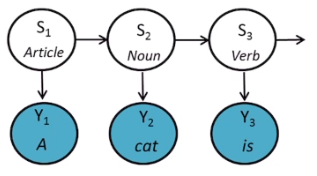
\includegraphics[scale=0.5]{27.png}
\end{center}
$S_i$ are \textbf{hidden states}, finite $i = 1,\ldots,C$.\\
We need \textbf{clustering algorithms}: clustering symbols into a finite set of non-observable elements.\\
Multinomial state transition
$$A_{ij} = P(S_t=i\:|\:S_{t-1}=j)$$
Prior probability (\textbf{stationary assumption})
$$\pi_i = P(S_1=i)$$
\textbf{Emission distribution} (the "down arrow" $\begin{array}{c}
S_t\\\downarrow\\Y_t
\end{array}$)
$$b_i(y_t) = P(Y_t = y_t\:|\:S_t = i)$$
\paragraph{HMM Joint Probability Factorization} Discrete state HMMs are parameterized by the finite number of hidden states $C$ and $\Theta = (\pi, A, B)$:
\begin{list}{}{}
	\item $\pi$ prior distribution
	\item $A$ state transition
	\item $B$ emission distribution (or its parameters)
\end{list}
$$P(Y = y) = \sum_s P(Y=y,S=s) =$$
$$= \sum_{s_1,\ldots,s_T}\left( P(S_1=s_1)P(Y_1=y_1\:|\:S_1=s_1)\prod_{t=2}^T P(S_t=s_t\:|\:S_{t-1} = s_{t-1})P(Y_t=y_t\:|\:S_t=s_t)\right)$$
\paragraph{HMMs as Recursive Models} A graphical framework describing how contextual information is recursiverly encoded by both probabilistic and neural models.
\begin{center}
	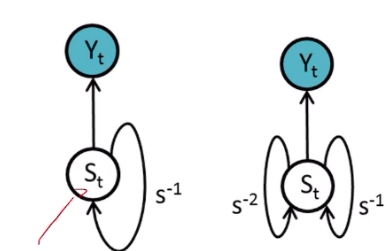
\includegraphics[scale=0.5]{28.png}
\end{center}
Indicates that the hidden state $S_t$ at time $t$ is dependent on context information from
\begin{list}{}{}
	\item the previous timestep $s^{-1}$, first-order
	\item the previous two timesteps $s^{-1},s^{-2}$, second-order
\end{list}
and so on.
\paragraph{HMMs as Automata} Can also be generalized to transducers.
\begin{center}
	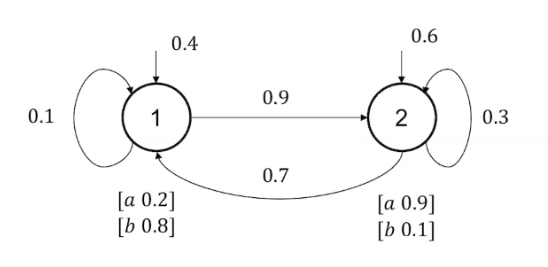
\includegraphics[scale=0.5]{29.png}
\end{center}
\pagebreak
\subsection{Notable Inference Problems}
\paragraph{Smoothing} Given a model $\Theta$ and an observed sequence $y$, determine the distribution of the hidden state at time $t$: $P(S_t\:|\:Y=y,\Theta)$\\
Forward Backward algorithm.
\paragraph{Learning} Given a dataset of $N$ sequences $D=\{y^1,\ldots,y^N\}$ and the number of hidden states $C$, find the parameters $\pi,A,B$ that maximize the probability model $\Theta = \{\pi,A,B\}$ having generated the sequences in $D$
\paragraph{Optimal State Assigment} Given a model $\Theta$ and an observed sequence $y$, find an optimal state assignment $s = s_1^*,\ldots,s_T^*$ for the hidden Markov chain.\\
Viterbi algorithm.
\subsubsection{Forward-Backward Algorithm} \textbf{Smoothing}: how do we determine $P(S_t = i\:|\:\hat{y})$? We will compute $P(S_t=i, \hat{y})$, it's proportional (just divide by $P(\hat{y})$).\\
I know $\Theta$, the model (its parameters). So I know $P(S_1) = \pi, P(S_t\:|\:S_{t-1} = A$ and $P(y_t\:|\:S_t) = B$: I need to express the quantity I want in terms of $\Theta=\{\pi,A,B\}$.\\
$\hat{y}$ are all the observations for each timestep $\Rightarrow P(S_t=i,y_1,\ldots,y_{t-1},y_t,y_{t+1},\ldots,y_T)$
$$S_1\rightarrow\ldots\rightarrow S_{t-1}\rightarrow S_t\rightarrow S_{t+1}\rightarrow\ldots\rightarrow S_T$$
$$\downarrow\rightarrow\ldots\rightarrow \downarrow\rightarrow \downarrow\rightarrow \downarrow\rightarrow\ldots\rightarrow \downarrow$$ %TODO format
$$y_1\rightarrow\ldots\rightarrow y_{t-1}\rightarrow y_t\rightarrow y_{t+1}\rightarrow\ldots\rightarrow y_T$$
We are at time $t$, so everything after that is the future ($y_{t+1:T}$), and everything up to $t$ included is the past ($y_{1:t}$).
$$P(S_t=i,y_1,\ldots,y_{t-1},y_t,y_{t+1},\ldots,y_T) = P(y_{t+1:T}\:|\:S_t=i, y_{1:t}) P(S_t=i,y_{1:t})$$
If I observe $S_t$ we block the path $y_{1:t}$, so $P(y_{t+1:T}\:|\:S_t=i, y_{1:t}) = P(y_{t+1:T}\:|\:S_t=i)$
$$P(S_t=i,y_1,\ldots,y_{t-1},y_t,y_{t+1},\ldots,y_T) = P(y_{t+1:T}\:|\:S_t=i) P(S_t=i,y_{1:t})$$
I can derive two "messages"
\begin{list}{}{}
	\item Past message $\alpha_t(i) = P(S_t=i,y_{1:t})$ (\textbf{forward recursion})
	\item Future message $\beta_t(i) = P(y_{t+1:T}\:|\:S_t=i)$ (\textbf{backward recursion})
\end{list}
$$P(S_t,y_{1:t}) = \sum_{j=1}^c P(S_t, S_{t-1}=j,y_{1:t}) = \sum_{j=1}^c P(y_t\:|\:S_t, S_{t-1} = j, y_{1:t-1})P(S_t,S_{t-1},y_{1:t-1})$$
But we can get rid of $S_{t-1}=j$ and $y_{1:t-1}$ leaving us with $P(y_t\:|\:S_t)$ which is just the emission.\\
The second factor can be rewrited as $P(S_t\:|\:S_{t-1}=j,y_{1:t-1}) P (S_{t-1}=j\:|\:y_{1:t-1})$ and observing $S_{t-1}$ allows us to get rid of $y_{1:t-1}$, giving us the transition distribution $P(S_t\:|\:S_{t-1}=j)$ and $\alpha_{t-1}(j)$
$$\alpha_t(i) = P(S_t=i,y_{1:t}) = \sum_{j=1}^c P(y_t\:|\:S_t=i) P(S_t=i\:|\:S_{t-1}=j)\alpha_{t-1}(j)$$
$$\alpha_1(j) = P(y_1\:|\:S_1=j)P(S_1=j)$$
This just by reasoning with conditional independence.\\
Same thing can be done for $$P(y_{t+1:T}\:|\:S_{t} = i) = \sum_j P(y_{t+1:T},S_{t+1}=j\:|\:S_t=i) = \sum_j P(y_{t+2:T}\:|\:S_t, S_{t+1},y_{t+1})P(S_{t+1},y_{t+1}\:|\:S_t=i)$$
Same as before, I can exclude $S_t, y_{t+1}$ because we observe $S_{t+1}$ so that factor is $\beta_{t+1}(j)$.\\
The second factor is rewritten as $P(S_{t+1}\:|\:S_t,y_{t+1})P(y_{t+1}\:|\:S_{t+1})$ which is the transition distribution (we can exclude $y_{t+1}$) times the emission distribution.
$$\beta_t(i) = \sum_j P(y_{t+1}\:|\:S_{t+1} = j)P(S_{t+1}=j\:|\:S_t=i)\beta_{t+1}(j)$$ %TODO check
$$\beta_T = 1$$
\paragraph{Sum-Product Message Passing} The Forward-Backward algorithm is an example of a sum-product message passing algorithm.\\
A forward recursion computing a generic message $\mu_\alpha$, backward recursion computing a generic message $\mu_\beta$\\
A general approach to efficiently perform exact inference in graphical models, with $\alpha_t \equiv \mu_\alpha(X_n)$ and $\beta_{t}\equiv \mu_\beta(X_n)$
$$\mu_\alpha(X_n) = \sum_{X_{n+1}} \psi(X_n, X_{n+1})\mu_\beta(X_{n+1})$$
\subsubsection{Learning in HMM}
Learning parameters $\Theta=(\pi,A,B)$ by \textbf{maximum} (log) \textbf{likelihood}
$$L(\Theta) = \log\prod_{n=1}^N P(Y^n\:|\:\Theta) = \log\prod_{n=1}^N\left(\sum_{S_1^n,\ldots,S_{T_n}^n} P(S_1^n)P(Y_1^n\:|\:S_1^n)\prod_{t=2}^T P(S_t^n\:|\:S_{t-1}^n)P(Y_t^n\:|\:S_t^n)\right)$$
Maximizing the joint likelihood of the sequences given the parameters considering them independent and identically distributed. We have to deal with the unobserved $S_t^n$ and the nasty sum in the log.\\
Expectation-Maximization of the \textbf{complete likelihood} $L_c(\Theta)$, optimizing a slightly different problem obtaining a not-reducing similar result. It's completed with indicator variables $z_{ti}^n=\left\{\begin{array}{c l}
1&\hbox{if }n\hbox{th chain is in state }i\hbox{ at time }t\\
0&\hbox{otherwise}
\end{array}\right.$ about the assignments $S_i^n$
\paragraph{Expectation-Maximization} Gives the red line: touching in the estimating point and not greater in the other points.
\begin{center}
	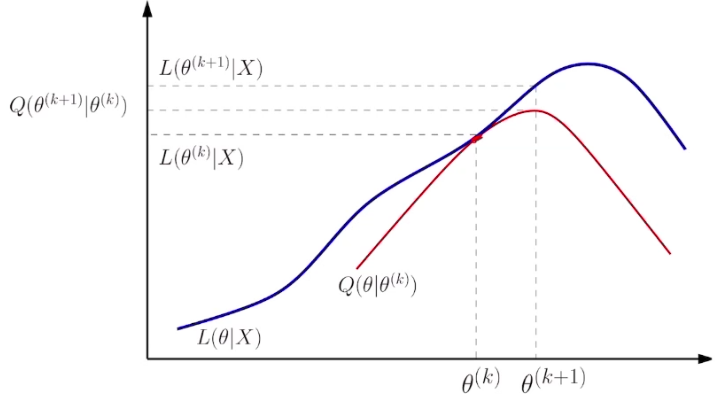
\includegraphics[scale=0.5]{30.png}
\end{center}
It's a matter of picking the right $Q(\Theta\:|\:\Theta^k)$\\
Introduce indicator variables in $L(\Theta)$ together with model parameters $\Theta = (\pi,A,B)$
$$L_C(\Theta)=\log P(X,Z\:|\:\Theta) =$$%TODO formulona p. 19
But I built it assuming to know $z$, but I don't know it. The \textit{expectation} part is in this: I don't know $z_{ti}^n$, but you can optimize the function in expectation $E[L_C(\Theta)]$\\
It's a 2-step iterative algorithm for the maximization of complete likelihood $L_C(\Theta)$ with respect to the model parameters $\Theta$\begin{list}{}{}
	\item E-step: given the current estimate of the model parameters $\Theta^t$, compute $$Q^{t+1}(\Theta\:|\:\Theta^t) = E_{Z\:|\:X,\Theta^t}[\log P(X,Z\:|\:Theta)]$$
	So compute the expectation of the complete log likelihood with respect to indicator variables\ldots %TODO
	Expectation with respect to a discrete random variable is $$E_z[Z] = \sum_z z\cdot P(Z=z)$$
	\item M-step: find the new estimate of the model parameters $$\Theta^{t+1} = \arg\max_\Theta Q^{t+1}(\Theta\:|\:\Theta^t)$$
\end{list}

\end{document}